\PassOptionsToPackage{off}{epstopdf}
\documentclass{article}

% NeurIPS 2024 style (used by ML4PhysicalSciences / AI4Science workshops).
% [final] = camera-ready (no line numbers); [preprint] = arXiv-friendly.
\usepackage[preprint]{neurips_2024}

% Override footer for ML4PhysicalSciences workshop, NeurIPS 2026.
\makeatletter
\renewcommand{\@noticestring}{%
  Workshop on Machine Learning for the Physical Sciences, NeurIPS 2026.%
}
\makeatother

\usepackage[utf8]{inputenc}
\usepackage[T1]{fontenc}
\usepackage{microtype}
\usepackage{amsmath,amssymb}
\usepackage{graphicx}
\usepackage{booktabs}
\usepackage{xcolor}
\usepackage{enumitem}
\setlist{itemsep=2pt,topsep=2pt}
\usepackage[font=small,labelfont=bf]{caption}
\usepackage{subcaption}
\captionsetup{aboveskip=4pt,belowskip=2pt}
\usepackage{tikz}
\usetikzlibrary{arrows.meta,positioning,calc}
\usepackage{pgfplots}
\pgfplotsset{compat=1.18}
\usepackage{hyperref}
\hypersetup{colorlinks=true,linkcolor=red!60!black,urlcolor=blue!60!black,citecolor=green!50!black}
\usepackage{cleveref}

% Tighten up for a 4-page budget.
\setlength{\textfloatsep}{6pt plus 1pt minus 1pt}
\setlength{\intextsep}{6pt plus 1pt minus 1pt}
\setlength{\dbltextfloatsep}{6pt plus 1pt minus 1pt}

\title{Physics-Gated Correction Discovery: Why Constraining the Search Space Beats Scaling It in Noisy Symbolic Regression}

\author{%
  Muhammad Afif Erdita \\
  Independent Researcher, Indonesia \\
  \texttt{maeapip10@gmail.com}
}

\begin{document}
\maketitle

\begin{abstract}
Symbolic regression (SR) methods such as PySR, AI~Feynman, and PhySO discover equations \emph{from scratch}, an approach that is sensitive to noisy physical data: under matched residuals, PySR's structural accuracy is non-monotonic in noise and does not improve when its search budget is doubled. We argue that scientific discovery is rarely \emph{tabula rasa}; it is \emph{correction-first}. Given a known classical law and anomalous data, the real task is to find the minimal physically-valid correction $\Delta$. We present \textbf{Anomaly-Driven Correction Discovery (ADCD)}, which restricts search to a correction subspace and cascades three physical filters (AST complexity, dimensional homogeneity with a transcendental-argument guardrail, and asymptotic-regime consistency [ARC]) \emph{before} a JAX optimizer fits any parameter, with Bayesian Information Criterion (BIC) reranking. On a 9-scenario benchmark (overall mean $80.4\%\pm7.4\%$ across 16 seeds and all noise levels; $88.9\%$ at the disclosed reference seed), ADCD reaches $88.9\%$ at $5\%$ noise versus $11.1\%$ for PySR, a \emph{seed-independent} gap: ADCD's \emph{worst} of 16 seeds still exceeds PySR with doubled budget. Removing all gates drops recovery by $44.5$\,pp. ADCD is orthogonal to, not competitive with, existing SR: it restricts the problem they solve to a physically-motivated subspace where unconstrained search is least reliable under noise.
\end{abstract}


%==================================================================
\section{Introduction}
\label{sec:intro}

When a physical law breaks down under extreme conditions, the scientific question is not ``what is the correct law?'' Instead, it is ``what is the \emph{minimal correction} to the known law?'' The dominant paradigm in symbolic regression (SR) answers a different question: it discovers $f(X)\approx y$ from a blank slate, an approach that, as we show, degrades under realistic noise. Pioneered by Eureqa~\cite{schmidt2009distilling}, AI~Feynman~\cite{udrescu2020ai}, and PySR~\cite{cranmer2020pysr}, and extended by deep RL approaches such as DSR~\cite{petersen2021deep} and unit-constrained PhySO~\cite{tenachi2023physo}, these systems recover compact laws in \emph{low}-noise regimes. Under realistic observational noise, however, their structural accuracy degrades and is often \emph{non-monotonic} in noise: a larger candidate pool does not reliably translate into the correct functional \emph{class} (\Cref{sec:exp}).

This difficulty stems in part from a limitation in \emph{problem formulation}. Science rarely discovers from a blank slate; it \emph{corrects}. From the relativistic kinetic-energy expansion $\tfrac12 mv^2(1+\tfrac34 v^2/c^2+\dots)$, to Debye-screened Coulomb potentials $V(r)\propto r^{-1}e^{-r/\lambda_D}$, to turbulent drag $F=bv+\alpha v^2$, progress takes a structurally-correct classical law and appends a \emph{minimal correction} $\Delta$ that reconciles it with anomalous data. This restricts the hypothesis space from the full function space $\mathcal{F}$ to a correction subspace $\mathcal{D}\subset\mathcal{F}$, an exponential reduction informed by the known physics.

The proposed \textbf{Anomaly-Driven Correction Discovery (ADCD)} framework introduces three main contributions:
\textbf{(C1) Correction-first paradigm:} Search for $\Delta$ in a restricted correction subspace $\mathcal{D} \subset \mathcal{F}$, not the full function space $f$ in $\mathcal{F}$, given a known classical law $y_{\rm classical}=g(X;\phi)$ and anomalous observations.
\textbf{(C2) Physics-gated cascade before optimization:} Three physical consistency filters (AST complexity, dimensional homogeneity, and asymptotic decoupling limits $\Delta \to 0$ at the classical boundary) screen candidates \emph{before} any parameter is numerically fit.
\textbf{(C3) Noise-robust stability:} ADCD's structural accuracy is monotonic in noise because it avoids the universal-approximator regime that overfits noise into nested mathematical structures.

We deliberately scope this paper to \emph{method and synthetic benchmark}; real-data validation (galactic, cosmological) is reported in a companion manuscript.

\begin{figure}[t]
\centering
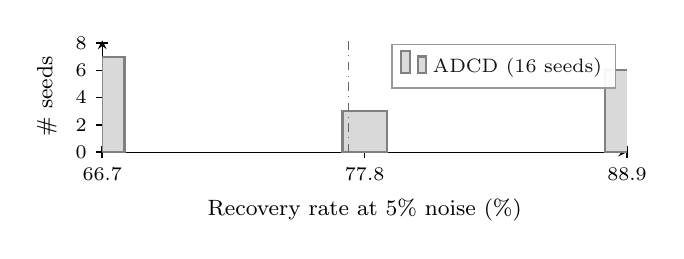
\begin{tikzpicture}
\begin{axis}[
  width=0.68\linewidth, height=3.0cm,
  ybar, bar width=16pt,
  xlabel={Recovery rate at $5\%$ noise (\%)},
  ylabel={\# seeds},
  ymin=0, ymax=8.2,
  xtick={66.7,77.8,88.9},
  xticklabels={66.7,77.8,88.9},
  ytick={0,2,4,6,8},
  enlarge x limits=0.28,
  axis lines=left,
  tick style={black, semithick},
  every axis label/.style={font=\footnotesize},
  tick label style={font=\scriptsize},
  legend style={font=\scriptsize, at={(0.98,0.97)}, anchor=north east,
                draw=black!40, fill=white, fill opacity=0.92, row sep=-1pt},
  legend cell align=left,
]
% ADCD per-seed counts at 5% noise: 66.7%->7, 77.8%->3, 88.9%->6 (16 seeds)
\addplot[fill=black!15, draw=black!50, thick] coordinates {
  (66.7,7) (77.8,3) (88.9,6)
};
% PySR reference lines
\draw[red!70!black, very thick, dashed] (axis cs:11.1,0) -- (axis cs:11.1,8.2);
\draw[red!70!black, thick, dotted]      (axis cs:55.6,0) -- (axis cs:55.6,8.2);
\draw[black!60, thin, dash dot]         (axis cs:77.1,0) -- (axis cs:77.1,8.2);
\legend{ADCD (16 seeds),PySR fair 11.1\%,PySR generous 55.6\%,ADCD mean 77.1\%}
\end{axis}
\end{tikzpicture}
\caption{Seed-independence of the ADCD-PySR gap at $5\%$ noise. Every one of ADCD's 16 seeds (bars) recovers at least $66.7\%$, above PySR's best result even under doubled budget ($55.6\%$, dotted).}
\label{fig:seeds}
\end{figure}

%==================================================================
\section{Related work}
\label{sec:related}

\paragraph{Tabula rasa symbolic regression.}
Modern SR discovers an expression $f(X)\!\approx\!y$ from a blank slate. Eureqa~\cite{schmidt2009distilling} pioneered genetic search over expression trees; AI~Feynman~\cite{udrescu2020ai} added concepts like symmetry and unit filtering; PySR~\cite{cranmer2020pysr} scaled genetic SR; DSR~\cite{petersen2021deep} applied reinforcement learning. All share a common limitation: under realistic noise their structural accuracy degrades and is often \emph{non-monotonic} in noise, because a larger search space rewards overfit structure rather than the correct functional class. ADCD departs by searching only the correction subspace $\mathcal{D}\!\subset\!\mathcal{F}$ to a \emph{known} law, an exponential restriction of the hypothesis space.

\paragraph{Unit-constrained \& LLM-guided SR.}
PhySO~\cite{tenachi2023physo} enforces dimensional homogeneity during RL training, while LaSR~\cite{grayeli2024lasr} uses language models to evolve a concept library. ADCD is complementary: its physics-gated cascade (dimensional, asymptotic, complexity) filters proposed candidates \emph{before} any numerical parameter optimization, regardless of whether they are generated by grammar or LLM samplers.

\paragraph{Physics in models vs.\ search space.}
Instead of baking physics into the loss (PINNs~\cite{raissi2019pinn}), coordinates (HNNs~\cite{greydanus2019hnn}), or differential equations (SINDy~\cite{champion2019sindy}), ADCD restricts the symbolic \emph{search space} directly. It provides interpretable, pre-fit filters that any downstream optimizer operates within.

\begin{figure}[t]
\centering
\begin{subfigure}[t]{0.48\linewidth}\centering

\includegraphics[width=\linewidth, height=2.3cm]{fig1_noise_robustness.pdf}
\caption{Noise robustness. ADCD stable; PySR fair non-monotonic (44$\to$56$\to$11$\to$56\%).}
\label{fig:noise}
\end{subfigure}\hfill
\begin{subfigure}[t]{0.48\linewidth}\centering

\includegraphics[width=\linewidth, height=2.3cm]{fig4_ablation.pdf}
\caption{Gate ablation at $5\%$ noise. Removing all gates collapses recovery by $44.5$\,pp.}
\label{fig:ablation}
\end{subfigure}
\caption{Left: structural match rate vs.\ noise. Right: per-gate ablation.}
\label{fig:both}
\end{figure}

%==================================================================
\section{The ADCD framework}
\label{sec:method}

\paragraph{Residual extraction.}
Given a known classical law $y_{\rm classical}=g(X;\phi)$ and noisy anomalous data $y_{\rm obs}$, ADCD isolates the correction by forming a residual. In \emph{multiplicative} mode $y_{\rm true}=y_{\rm classical}(1+\Delta)$ gives $\delta=y_{\rm obs}/y_{\rm classical}-1$; in \emph{additive} mode $y_{\rm true}=y_{\rm classical}+\Delta$ gives $\delta=y_{\rm obs}-y_{\rm classical}$. A mode selector picks whichever best isolates the anomalous deviation.

\paragraph{Proposer.}
Candidate correction templates $\Delta(X;\theta)$ are drawn from a stochastic sampler over dimensionless ratios, biased by residual features (monotonicity, curvature, oscillation, exponential decay $R^2$, symmetry) that upweight plausible families but never gate candidates; only the physics cascade does.

\paragraph{Stage 1: cascaded physics gates.}
Every candidate passes three physical filters \emph{before} parameter fitting:
\textbf{G1. AST complexity:} Reject expressions with AST depth $>7$ or $>20$ tokens (Occam prior).
\textbf{G2. Dimensional homogeneity:} Verify $\Delta$ is dimensionless; physical variables enter only inside dimensionless ratios, and transcendental arguments (e.g., inside $\exp$, $\sin$) must be dimensionless.
\textbf{G3. Asymptotic-regime consistency (ARC):} Enforce the decoupling limit: $\lim_{x\to x_0}\Delta(X;\theta)=0$ (e.g., $v\to 0$ or $r\to \infty$) evaluated via SymPy.
Survivors are coarsely ranked by preliminary NMSE on $\delta$, giving an early data-driven signal before the full fit.

\paragraph{Stage 2: JAX-traced optimization + BIC reranking.}
Surviving expressions are transpiled to JAX and fit by L-BFGS-B (multi-restart, log-uniform init) minimizing NMSE of the residual:
$\text{NMSE}=\tfrac{\sum_i(\Delta(X_i;\theta)-\delta_i)^2}{\sum_i(\delta_i-\bar\delta)^2}$.
Under noise, flexible wrong-class expressions can achieve lower NMSE than the truth, so we rerank by the Bayesian Information Criterion~\cite{schwarz1978bic,rissanen1978mdl}: $\text{BIC}=N\ln(\text{NMSE})+k\ln N$, whose $k\ln N$ penalty selects parsimonious correct-class forms. The winner is classified into one of six families by AST traversal, with degenerate-exponent detection.

\begin{figure}[t]
\centering
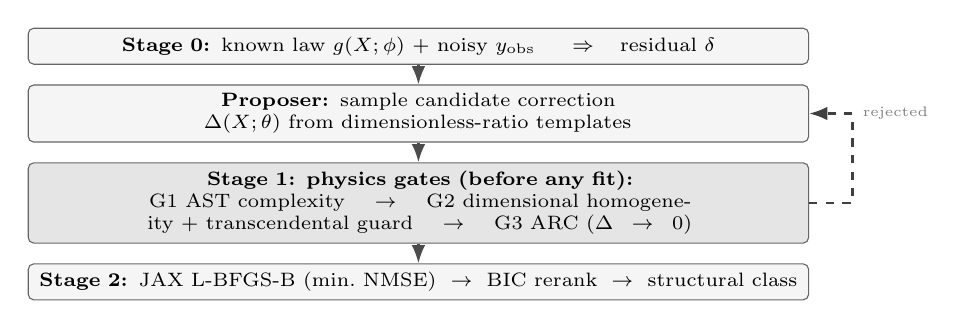
\begin{tikzpicture}[node distance=0.25cm,
  block/.style={rectangle,draw=black!60,rounded corners=2pt,fill=black!4,
                text width=0.80\linewidth,inner sep=3pt,align=center,font=\scriptsize},
  gate/.style={rectangle,draw=black!60,rounded corners=2pt,fill=black!10,
               text width=0.80\linewidth,inner sep=3pt,align=center,font=\scriptsize},
  line/.style={draw,-Latex,thick,gray!60!black},
  fb/.style={draw,-Latex,thick,gray!50!black,dashed}]
\node[block] (s0)   {\textbf{Stage 0:} known law $g(X;\phi)$ + noisy $y_{\rm obs}\;\Rightarrow\;$ residual $\delta$};
\node[block,below=of s0]   (prop) {\textbf{Proposer:} sample candidate correction $\Delta(X;\theta)$ from dimensionless-ratio templates};
\node[gate,below=of prop]  (g)   {\textbf{Stage 1: physics gates (before any fit):}\\
   G1 AST complexity $\;\to\;$ G2 dimensional homogeneity + transcendental guard $\;\to\;$ G3 ARC ($\Delta\!\to\!0$)};
\node[block,below=of g]    (opt) {\textbf{Stage 2:} JAX L-BFGS-B (min.\ NMSE) $\;\to\;$ BIC rerank $\;\to\;$ structural class};
\path[line] (s0)   -- (prop);
\path[line] (prop) -- (g);
\path[line] (g)    -- (opt);
% rejected candidates loop back to the proposer, routed clear of all boxes
\path[fb] (g.east) -- ++(0.55,0) |- node[font=\tiny,gray,right,pos=0.5]{rejected} (prop.east);
\end{tikzpicture}
\caption{ADCD pipeline. Physics gates (G1--G3) screen candidates \emph{before} any parameter is fit; rejected candidates are re-sampled.}
\label{fig:pipeline}
\vspace{-4pt}
\end{figure}

\paragraph{Relation to EFT.}
The cascade mirrors the correction-first philosophy of Effective Field Theory~\cite{weinberg1979eft}: dimensional analysis of operators (G2), decoupling of heavy modes in the low-energy limit (G3/ARC), and power counting (BIC). ADCD has no renormalization-group flow or controlled $E/\Lambda$ expansion; instead, it \emph{automates} that philosophy for data-driven problems.

%==================================================================
\section{Experiments}
\label{sec:exp}

\paragraph{Benchmark.}
We evaluate on 9 physical-anomaly scenarios in three tiers: \emph{textbook} (relativistic KE, Yukawa gravity, anharmonic spring), \emph{cross-domain} (net radiation $T^{-4}$, nonlinear drag, screened Coulomb), and \emph{synthetic novel} formulas. Each is run at $0/1/5/10\%$ observational noise. Success = correct structural \emph{class} recovery (e.g.\ discovering an exponential correction where the truth is exponential). We report a 16-seed distribution; the mean is the primary claim and seed=42 (the highest seed) is disclosed explicitly, never as the headline.

\paragraph{Baselines.}
We compare against PySR~\cite{cranmer2020pysr} on the \emph{same residual targets} $\delta=y_{\rm obs}-y_{\rm classical}$. The primary baseline is the \texttt{fair} profile ($n_{\rm iter}{=}100$, \texttt{maxsize}{=}30, 60\,s/scenario). To rule out a budget artefact we add a \texttt{generous} profile that \emph{doubles} every budget axis ($n_{\rm iter}{=}200$, \texttt{maxsize}{=}40, 120\,s; $\sim3\times$ wall-clock).

\paragraph{Main result: the gap is structural, not budgetary.}
\Cref{tab:baseline} reports structural match rates. ADCD reaches $88.9\%$ (8/9) at $5\%$ noise versus $11.1\%$ (1/9) for PySR fair, representing a $77.8$\,pp gap under matched residuals. The comparison is \emph{seed-independent}: at $5\%$ noise ADCD's worst of 16 seeds ($66.7\%$, 6/9; cf.\ the per-seed distribution in our bundled artefacts) still exceeds PySR fair. Doubling PySR's budget does \emph{not} close the gap; \texttt{generous} total recovery stays flat at $15/36$ (identical to \texttt{fair}) and at the $5\%$ headline point it reaches only $5/9$ ($55.6\%$). The extra budget explores deeper trees (mean complexity $9.8$ vs.\ $8.7$ nodes) spent on more deeply-overfit rather than more physically-correct structure. The binding constraint is \emph{structural selection}, not search budget; physics gates resolve it directly.

\begin{table}[h]
\centering
\small
\caption{Structural class match rate on the 9-scenario residual benchmark. \texttt{generous} doubles PySR's budget on every axis yet does not close the gap.}
\label{tab:baseline}
\begin{tabular}{lcccc}
\toprule
\textbf{Method} & \textbf{0\%} & \textbf{1\%} & \textbf{5\%} & \textbf{10\%} \\
\midrule
ADCD (ours, seed=42) & 9/9 (100\%) & 9/9 (100\%) & \textbf{8/9 (88.9\%)} & 8/9 (88.9\%) \\
ADCD 16-seed mean    & 86.8\% & 81.3\% & \textit{77.1\%$\pm$10.0\%} & 76.4\% \\
PySR fair            & 4/9 (44.4\%) & 5/9 (55.6\%) & 1/9 (11.1\%) & 5/9 (55.6\%) \\
PySR generous ($2\times$) & 4/9 (44.4\%) & 4/9 (44.4\%) & 5/9 (55.6\%) & 2/9 (22.2\%) \\
\bottomrule
\end{tabular}
\end{table}

The seed-independence of this gap is structural, not artefactual. \Cref{fig:seeds} bins ADCD's per-seed recovery at the $5\%$ headline noise level: the entire 16-seed distribution sits between $66.7\%$ and $88.9\%$, \emph{entirely above} PySR's best result even under doubled budget ($55.6\%$, \texttt{generous}). ADCD's worst seed exceeds PySR's best by $11.1$\,pp; the gap cannot be attributed to a favourable seed choice.

\paragraph{Why PySR is non-monotonic, and why ADCD is not.}
PySR fair's accuracy is non-monotonic in noise ($4,5,1,5$ out of 9) because at $0\%$ noise it overfits to complex trigonometric structures (mean $13.8$ nodes). ADCD avoids this because its physical gates are noise-independent: dimensional and ARC filters reject overfit structures before optimization, allowing robust selection across all SNRs (\Cref{fig:noise}).

\paragraph{Ablation: the gates act collectively.}
Disabling gates one at a time at $5\%$ noise (\Cref{fig:ablation}) shows that removing ARC, AST, or the coarse-eval pre-filter leaves accuracy unchanged ($8/9$), while disabling the dimensional gate alone costs $11.1$\,pp ($8/9\to7/9$). Disabling all gates collapses performance ($8/9\to4/9$, $-44.5$\,pp), showing that the gates act collectively to enforce physical consistency.

%==================================================================
\section{Discussion and limitations}
\label{sec:disc}

\paragraph{ADCD is a restriction, not a competitor.}
ADCD does not compete with PhySO or PySR; it restricts the problem they solve to a physically-motivated subspace where unconstrained search is least reliable under noise. This makes ADCD directly \emph{combinable} with them: a PhySO/PySR/LaSR~\cite{grayeli2024lasr} proposer could feed the same gate cascade.

\paragraph{Honest limitations and proposer template bias.}
ADCD assumes a structurally-correct classical baseline (incremental correction, not wholesale replacement). Under high noise ($\ge 5\%$), screened-Coulomb decay is fitted by a rational proxy, reflecting decay-vs-saturation ambiguity under limited dynamic range. 
Crucially, the current proposer layer (whether grammar- or LLM-driven) is fundamentally bottlenecked by \emph{prior template bias}: it samples candidate corrections from a predefined dictionary of known functional families. This restricts the search space to mathematical structures already documented in human physics literature, leaving the framework unable to discover truly unexpected or non-templated functional corrections.

\paragraph{The breakthrough path: complete functional bases.}
To escape this template bottleneck, our ongoing work focuses on replacing heuristic templates with a systematic, non-templated expansion. By applying the Buckingham-$\Pi$ theorem to the system variables, we construct independent dimensionless groups ($\Pi_1, \Pi_2, \dots$), and expand the correction $\Delta$ directly in a \emph{complete functional basis} (e.g., Chebyshev polynomials, Legendre polynomials, or Bessel series) defined over these groups. This shifts the paradigm from "rediscovering known families" to a systematic mathematical search over complete function spaces, ensuring that unexpected physics can be captured without prior bias.

\paragraph{Reproducibility and fail-safe behavior.}
ADCD ships as an open-source Python package with a JAX backend, public CLI, and bundled test seeds. Unlike GPU-intensive frameworks, it runs in seconds on consumer CPUs, making replication accessible without HPC resources. On a 6-case misspecification benchmark, it fails to converge rather than outputting confident spurious equations, establishing a crucial fail-safe property.

\paragraph{AI disclosure.} Large language models assisted in code development and manuscript drafting under human guidance. The human author conceived the hypotheses, designed the experiments, verified all findings, and remains fully responsible for the work.

\paragraph{Closing.}
Noisy symbolic regression is bottlenecked by \emph{structural selection}, not search budget. The correction-first formulation, which searches for a physically-valid $\Delta$ to a known law screened by dimensional and asymptotic gates before any fit, resolves this directly: ADCD delivers seed-independent gains over PySR, stays robust where unconstrained search is non-monotonic, and is orthogonal to existing SR systems. Future work extends the cascade to multivariable laws and integrates it as a selection layer over external proposers (PhySO, LaSR).

%==================================================================
\bibliographystyle{plainnat}
\begin{thebibliography}{12}
\scriptsize
\setlength{\itemsep}{0pt}
\bibitem[Schmidt \& Lipson(2009)]{schmidt2009distilling}
M.~Schmidt \& H.~Lipson.
\newblock Distilling free-form natural laws from experimental data.
\newblock \emph{Science}, 324(5923):81--85, 2009.

\bibitem[Udrescu \& Tegmark(2020)]{udrescu2020ai}
S.~M. Udrescu \& M.~Tegmark.
\newblock AI Feynman: A physics-inspired systematic approach to symbolic regression.
\newblock \emph{Science Advances}, 6(16), 2020.

\bibitem[Cranmer(2020)]{cranmer2020pysr}
M.~Cranmer.
\newblock PySR: Fast \& parallelized symbolic regression in Python/Julia.
\newblock \emph{arXiv:2007.03738}, 2020.

\bibitem[Petersen et~al.(2021)]{petersen2021deep}
B.~K. Petersen et~al.
\newblock Deep symbolic regression: Recovering mathematical expressions from data via risk-seeking policy gradients.
\newblock In \emph{ICLR}, 2021.

\bibitem[Tenachi et~al.(2023)]{tenachi2023physo}
W.~Tenachi, R.~Ibata, \& F.~I. Diakogiannis.
\newblock Deep symbolic regression for physics guided by units constraints.
\newblock \emph{Astrophysical Journal}, 959(2):99, 2023.

\bibitem[Grayeli et~al.(2024)]{grayeli2024lasr}
A.~Grayeli, A.~Sehgal, O.~Costilla-Reyes, M.~Cranmer, \& S.~Chauduri.
\newblock Symbolic regression with a learned concept library.
\newblock In \emph{NeurIPS}, 2024.

\bibitem[Schwarz(1978)]{schwarz1978bic}
G.~Schwarz.
\newblock Estimating the dimension of a model.
\newblock \emph{Annals of Statistics}, 6(2):461--464, 1978.

\bibitem[Rissanen(1978)]{rissanen1978mdl}
J.~Rissanen.
\newblock Modeling by shortest data description.
\newblock \emph{Automatica}, 14(5):465--471, 1978.

\bibitem[Weinberg(1979)]{weinberg1979eft}
S.~Weinberg.
\newblock Phenomenological Lagrangians.
\newblock \emph{Physica A}, 96(1-2):327--340, 1979.

\bibitem[Raissi et~al.(2019)]{raissi2019pinn}
M.~Raissi, P.~Perdikaris, \& G.~E. Karniadakis.
\newblock Physics-informed neural networks: A deep-learning framework for solving forward and inverse problems involving nonlinear partial differential equations.
\newblock \emph{Journal of Computational Physics}, 378:686--707, 2019.

\bibitem[Greydanus et~al.(2019)]{greydanus2019hnn}
S.~Greydanus, M.~Dzamba, \& J.~Yosinski.
\newblock Hamiltonian neural networks.
\newblock In \emph{NeurIPS}, 2019.

\bibitem[Champion et~al.(2019)]{champion2019sindy}
K.~Champion, B.~Lusch, J.~N. Kutz, \& S.~L. Brunton.
\newblock Data-driven discovery of coordinates and governing equations.
\newblock \emph{Proceedings of the National Academy of Sciences}, 116(45):22445--22451, 2019.
\end{thebibliography}

\end{document}
